\documentclass[12pt,hyperref,a4paper,UTF8]{ctexart}
\usepackage{HDUReport}
\usepackage{listings}
\usepackage{xcolor}
\usepackage{graphicx}
\usepackage{setspace}
\usepackage{float}
\usepackage{amsmath}
\usepackage{amssymb}
\usepackage{booktabs}
\usepackage{multirow}
\setstretch{1.5}

\usepackage{enumitem}
\setlist[itemize]{itemsep=0pt, parsep=0pt}

\setmainfont{Times New Roman}

% 代码样式设置
\lstset{
    language=Verilog,
    basicstyle=\ttfamily\small,
    keywordstyle=\color{blue}\bfseries,
    commentstyle=\color{green!60!black},
    stringstyle=\color{red},
    numbers=left,
    numberstyle=\tiny\color{gray},
    stepnumber=1,
    numbersep=5pt,
    backgroundcolor=\color{gray!10},
    frame=single,
    rulecolor=\color{black!30},
    tabsize=4,
    breaklines=true,
    breakatwhitespace=true,
    showstringspaces=false,
    captionpos=b,
    xleftmargin=2em,
    framexleftmargin=1.5em
}

\usepackage{tikz}
\usetikzlibrary{shapes.geometric, arrows, positioning, arrows.meta, calc}

%封面页设置
{   
    \title{ 
        \vspace{1cm}
        \heiti \Huge \textbf{《电子信息技术虚拟仿真综合实践B》综合实验报告} \par
        \vspace{1cm} 
        \heiti \Large {\underline{基于Sobel/Prewitt算子的FPGA边缘检测图像处理}   }     
    }

    \author{
        \kaishu\Large 指导教师\ \dlmu[9cm]{高宇}  \\
        \kaishu\Large 学生姓名\ \dlmu[9cm]{陈文轩} \\
        \kaishu\Large 学生学号\ \dlmu[9cm]{23040447} \\
        \kaishu\Large 学生班级\ \dlmu[9cm]{23186011} \\
        \kaishu\Large 学生专业\ \dlmu[9cm]{智能硬件与系统(电子信息工程)} \qquad  \\
    }
        
    \date{\today}
}

\begin{document}

\cover
\thispagestyle{empty}

\newpage
\setcounter{page}{1}

%% 摘要与关键词
\begin{center}
\heiti\Large 摘\quad 要
\end{center}

本实验基于FPGA平台实现了图像边缘检测系统，采用Sobel和Prewitt两种经典边缘检测算子，对存储在ROM中的图像进行实时处理并在LCD屏幕上显示。系统采用流水线架构，实现了从原始RGB图像到边缘检测结果的完整处理链路，包括坐标映射与图像缩放、RGB转灰度预处理、3×3像素窗口构建以及卷积运算等核心功能模块。

实验参考OpenCV图像处理库的算法原理，将软件函数硬件化（Soft Core Hardening），在FPGA上实现了与\texttt{cv::Sobel()}和Prewitt算子等效的硬件加速处理。通过拨码开关可实时切换不同的边缘检测算法，直观对比各算法的检测效果。本设计还针对梯度幅值计算中绝对值和近似法存在的45°方向边缘高估问题，提出了加权近似法的优化方案。

\vspace{0.5cm}
\noindent\textbf{关键词：}FPGA；边缘检测；Sobel算子；Prewitt算子；图像处理；硬件加速

\newpage

\section{系统方案}

\subsection{系统原理介绍}

边缘检测是图像处理中的基础操作，其核心思想是检测图像中灰度值发生急剧变化的位置。在数学上，边缘对应于图像灰度函数的一阶导数极大值点或二阶导数过零点。

本系统采用基于梯度的边缘检测方法，使用Sobel和Prewitt两种算子计算图像的水平和垂直方向梯度，通过梯度幅值判断边缘强度。系统整体架构如图\ref{fig:system_arch}所示。

\begin{figure}[H]
\centering
\begin{tikzpicture}[
    node distance=1.2cm and 1.5cm,
    block/.style={rectangle, draw, fill=blue!20, text width=2.5cm, text centered, minimum height=1cm, rounded corners},
    arrow/.style={-Stealth, thick}
]
    % 上层3个模块
    \node[block] (coord) {坐标映射\\(缩放算法)};
    \node[block, right=of coord] (rom) {ROM读取\\(原始像素)};
    \node[block, right=of rom] (gray) {灰度转换\\(预处理)};
    
    % 下层2个模块
    \node[block, below=of coord, xshift=2.25cm] (edge) {边缘检测\\(算法选择)};
    \node[block, right=of edge] (out) {像素输出\\(LCD显示)};
    
    % 连接箭头
    \draw[arrow] (coord) -- (rom);
    \draw[arrow] (rom) -- (gray);
    \draw[arrow] (gray.south) -- ++(0,-0.5) -| (edge.north);
    \draw[arrow] (edge) -- (out);
\end{tikzpicture}
\caption{系统架构框图}
\label{fig:system_arch}
\end{figure}

\subsection{方案论证与比较}

\subsubsection{边缘检测算子比较}

表\ref{tab:operator_compare}对比了Sobel和Prewitt两种边缘检测算子的特性。

\begin{table}[H]
\centering
\caption{Sobel与Prewitt算子特性对比}
\label{tab:operator_compare}
\begin{tabular}{cccc}
\toprule
\textbf{特性} & \textbf{Sobel算子} & \textbf{Prewitt算子} \\
\midrule
中心行权重 & 2 & 1 \\
对噪声敏感度 & 较低 & 较高 \\
边缘平滑度 & 更平滑 & 更锐利 \\
计算复杂度 & 需要移位操作 & 仅需加法 \\
适用场景 & 噪声较多的图像 & 清晰图像 \\
\bottomrule
\end{tabular}
\end{table}

\subsubsection{梯度幅值计算方法比较}

精确的梯度幅值计算公式为：
\begin{equation}
|G| = \sqrt{G_x^2 + G_y^2}
\end{equation}

由于FPGA中实现平方根运算消耗大量资源，本设计采用绝对值和近似：
\begin{equation}
|G| \approx |G_x| + |G_y|
\end{equation}

表\ref{tab:gradient_compare}对比了不同梯度幅值计算方法的特性。

\begin{table}[H]
\centering
\caption{梯度幅值计算方法对比}
\label{tab:gradient_compare}
\begin{tabular}{cccc}
\toprule
\textbf{方法} & \textbf{公式} & \textbf{45°误差} & \textbf{资源消耗} \\
\midrule
精确计算 & $\sqrt{G_x^2+G_y^2}$ & 0\% & 最高 \\
绝对值和 & $|G_x|+|G_y|$ & +41\% & 最低 \\
最大值法 & $\max(|G_x|,|G_y|)$ & -29\% & 低 \\
加权近似 & $\max + \frac{\min}{2}$ & ±12\% & 中等 \\
\bottomrule
\end{tabular}
\end{table}

\section{各模块详细设计方法与思路}

\subsection{坐标映射与图像缩放模块}

本模块实现将LCD屏幕坐标映射到原始图像坐标，采用最近邻插值算法实现4倍放大显示。

\textbf{参数配置：}

（1）原始图像尺寸：100×100像素

（2）显示尺寸：400×400像素（4倍放大）

（3）屏幕分辨率：800×480像素

（4）图像居中位置：(200, 40)

\textbf{最近邻插值原理：}

最近邻插值是最简单的图像缩放算法，其核心思想是：对于目标图像中的每个像素点，直接找到其在源图像中对应的最近像素点，将该像素值作为目标像素值。

在4倍放大的场景下，目标图像的坐标范围为$[0, 399]$，需要映射到源图像坐标范围$[0, 99]$。设目标图像坐标为$dst\_coord$，源图像坐标为$src\_coord$，缩放因子为$scale\_factor=4$，则映射关系为：
\begin{equation}
src\_coord = \lfloor \frac{dst\_coord}{scale\_factor} \rfloor = \lfloor \frac{dst\_coord}{4} \rfloor
\end{equation}

其中$\lfloor \cdot \rfloor$表示向下取整。例如，目标坐标$dst\_coord \in [0,3]$映射到源坐标$src\_coord=0$，$dst\_coord \in [4,7]$映射到$src\_coord=1$，以此类推。这样，每个源像素被复制到$4 \times 4 = 16$个目标像素位置。

在硬件实现中，由于$4 = 2^2$，除以4的运算可以通过右移2位实现，即$dst\_coord >> 2$，无需使用除法器，极大地节省了硬件资源。

\begin{lstlisting}[caption={坐标映射模块代码}]
// 计算相对于放大图像的坐标
wire [10:0] rel_x_scaled = x_pos - IMG_X;  // 0~399
wire [10:0] rel_y_scaled = y_pos - IMG_Y;  // 0~399

// 最近邻插值：除以缩放因子4（右移2位）
wire [6:0] src_x = rel_x_scaled[8:2];  // 0~99
wire [6:0] src_y = rel_y_scaled[8:2];  // 0~99

// ROM地址计算
assign rom_addr = src_y * 100 + src_x;  // 0~9999
\end{lstlisting}

\subsection{RGB转灰度模块}

边缘检测算法通常在灰度图像上进行，因此需要将RGB彩色图像转换为灰度图像。

\textbf{参考OpenCV函数：}\texttt{cv::cvtColor(src, gray, COLOR\_RGB2GRAY)}

\textbf{标准灰度化公式：}
\begin{equation}
Gray = 0.299 \times R + 0.587 \times G + 0.114 \times B
\end{equation}

\textbf{FPGA定点优化：}

由于FPGA中浮点运算需要消耗大量逻辑资源且延迟较高，因此采用定点整数近似方法。将浮点系数乘以$256 = 2^8$并取整，得到整数系数：

$0.299 \times 256 \approx 77$，$0.587 \times 256 \approx 150$，$0.114 \times 256 \approx 29$

定点灰度化公式为：
\begin{equation}
Gray = \frac{77 \times R + 150 \times G + 29 \times B}{256}
\end{equation}

其中除以256可通过右移8位实现，即取计算结果的高8位。

系数验证：$77/256 \approx 0.301$，$150/256 \approx 0.586$，$29/256 \approx 0.113$，与标准系数误差均小于1\%，满足工程精度要求。

\begin{lstlisting}[caption={RGB转灰度模块代码}]
wire [7:0] r = rom_data[23:16];
wire [7:0] g = rom_data[15:8];
wire [7:0] b = rom_data[7:0];

wire [15:0] gray_calc = r * 77 + g * 150 + b * 29;
wire [7:0] gray = gray_calc[15:8];  // 右移8位 = 除以256
\end{lstlisting}

\subsection{3×3像素窗口构建模块}

边缘检测卷积运算需要获取当前像素及其8邻域像素，形成3×3窗口。

\textbf{窗口结构：}
\begin{equation}
\begin{bmatrix} p_{00} & p_{01} & p_{02} \\ p_{10} & p_{11} & p_{12} \\ p_{20} & p_{21} & p_{22} \end{bmatrix}
\end{equation}

\textbf{实现原理：}

（1）使用两个行缓存\texttt{line\_buf0}和\texttt{line\_buf1}存储前两行的灰度值

（2）当前行使用移位寄存器实时获取

（3）每个时钟周期，9个像素值同时更新，形成完整的3×3窗口

\begin{lstlisting}[caption={3×3窗口构建代码}]
// 行缓存
reg [7:0] line_buf0 [0:IMG_WIDTH-1];  // 前2行缓存
reg [7:0] line_buf1 [0:IMG_WIDTH-1];  // 前1行缓存

// 窗口构建逻辑
always @(posedge lcd_clk) begin
    if (in_image_d1) begin
        // 从行缓存读取并移位
        p02 <= p01; p01 <= p00; p00 <= line_buf0[src_x_d1];
        p12 <= p11; p11 <= p10; p10 <= line_buf1[src_x_d1];
        p22 <= p21; p21 <= p20; p20 <= gray;
        
        // 更新行缓存
        line_buf0[src_x_d1] <= line_buf1[src_x_d1];
        line_buf1[src_x_d1] <= gray;
    end
end

// 窗口有效标志
wire window_valid = in_image_d3 && (src_x_d3 >= 7'd2) && (src_y_d3 >= 7'd2);
\end{lstlisting}

\subsection{Sobel边缘检测模块}

\textbf{参考OpenCV函数：}\texttt{cv::Sobel(src, dst, ddepth, dx, dy)}

\textbf{Sobel算子定义：}
\begin{equation}
G_x = \begin{bmatrix} -1 & 0 & +1 \\ -2 & 0 & +2 \\ -1 & 0 & +1 \end{bmatrix} \quad
G_y = \begin{bmatrix} -1 & -2 & -1 \\ 0 & 0 & 0 \\ +1 & +2 & +1 \end{bmatrix}
\end{equation}

\textbf{卷积计算公式：}
\begin{align}
G_x &= (p_{02} - p_{00}) + 2 \times (p_{12} - p_{10}) + (p_{22} - p_{20}) \\
G_y &= (p_{00} + 2 \times p_{01} + p_{02}) - (p_{20} + 2 \times p_{21} + p_{22})
\end{align}

\textbf{梯度幅值：}
\begin{equation}
|G| = |G_x| + |G_y|
\end{equation}

\begin{lstlisting}[caption={Sobel边缘检测代码}]
// Sobel Gx 计算: 水平方向梯度
wire signed [10:0] sobel_gx_row0 = $signed({3'b0, p02}) - $signed({3'b0, p00});
wire signed [10:0] sobel_gx_row1 = ($signed({3'b0, p12}) - $signed({3'b0, p10})) <<< 1;
wire signed [10:0] sobel_gx_row2 = $signed({3'b0, p22}) - $signed({3'b0, p20});
wire signed [11:0] sobel_gx = sobel_gx_row0 + sobel_gx_row1 + sobel_gx_row2;

// Sobel Gy 计算: 垂直方向梯度
wire signed [10:0] sobel_gy_top = $signed({3'b0, p00}) + ($signed({3'b0, p01}) <<< 1) + $signed({3'b0, p02});
wire signed [10:0] sobel_gy_bot = $signed({3'b0, p20}) + ($signed({3'b0, p21}) <<< 1) + $signed({3'b0, p22});
wire signed [11:0] sobel_gy = sobel_gy_top - sobel_gy_bot;

// 梯度幅值
wire [11:0] sobel_gx_abs = (sobel_gx < 0) ? -sobel_gx : sobel_gx;
wire [11:0] sobel_gy_abs = (sobel_gy < 0) ? -sobel_gy : sobel_gy;
wire [12:0] sobel_mag_full = sobel_gx_abs + sobel_gy_abs;

// 归一化到8位
wire [7:0] sobel_mag = (sobel_mag_full > 13'd2040) ? 8'd255 : sobel_mag_full[10:3];

// 阈值化输出 (白底黑边)
wire [23:0] data_sobel = (window_valid && sobel_mag > 8'd30) ? 24'h000000 : 24'hFFFFFF;
\end{lstlisting}

\subsection{Prewitt边缘检测模块}

\textbf{Prewitt算子定义：}
\begin{equation}
G_x = \begin{bmatrix} -1 & 0 & +1 \\ -1 & 0 & +1 \\ -1 & 0 & +1 \end{bmatrix} \quad
G_y = \begin{bmatrix} -1 & -1 & -1 \\ 0 & 0 & 0 \\ +1 & +1 & +1 \end{bmatrix}
\end{equation}

\textbf{卷积计算公式：}
\begin{align}
G_x &= (p_{02} - p_{00}) + (p_{12} - p_{10}) + (p_{22} - p_{20}) \\
G_y &= (p_{00} + p_{01} + p_{02}) - (p_{20} + p_{21} + p_{22})
\end{align}

Prewitt算子与Sobel算子的主要区别在于中心行的权重为1而非2，因此对噪声更敏感，但边缘更锐利。

\begin{lstlisting}[caption={Prewitt边缘检测代码}]
// Prewitt Gx 计算: 均匀权重
wire signed [10:0] prewitt_gx_row0 = $signed({3'b0, p02}) - $signed({3'b0, p00});
wire signed [10:0] prewitt_gx_row1 = $signed({3'b0, p12}) - $signed({3'b0, p10});
wire signed [10:0] prewitt_gx_row2 = $signed({3'b0, p22}) - $signed({3'b0, p20});
wire signed [11:0] prewitt_gx = prewitt_gx_row0 + prewitt_gx_row1 + prewitt_gx_row2;

// Prewitt Gy 计算: 均匀权重
wire signed [10:0] prewitt_gy_top = $signed({3'b0, p00}) + $signed({3'b0, p01}) + $signed({3'b0, p02});
wire signed [10:0] prewitt_gy_bot = $signed({3'b0, p20}) + $signed({3'b0, p21}) + $signed({3'b0, p22});
wire signed [11:0] prewitt_gy = prewitt_gy_top - prewitt_gy_bot;

// 梯度幅值
wire [11:0] prewitt_gx_abs = (prewitt_gx < 0) ? -prewitt_gx : prewitt_gx;
wire [11:0] prewitt_gy_abs = (prewitt_gy < 0) ? -prewitt_gy : prewitt_gy;
wire [12:0] prewitt_mag_full = prewitt_gx_abs + prewitt_gy_abs;

// 归一化到8位
wire [7:0] prewitt_mag = (prewitt_mag_full > 13'd1530) ? 8'd255 : prewitt_mag_full[10:3];

// 阈值化输出 (白底黑边)
wire [23:0] data_prewitt = (window_valid && prewitt_mag > 8'd25) ? 24'h000000 : 24'hFFFFFF;
\end{lstlisting}

\section{电路设计（Verilog HDL设计）}

\subsection{整体设计}

系统采用模块化设计，主要包含以下功能模块：

（1）\textbf{lcd\_pll}：时钟PLL模块，将50MHz系统时钟分频为33MHz LCD驱动时钟

（2）\textbf{lcd\_driver}：LCD驱动模块，生成LCD时序信号

（3）\textbf{lcd\_display}：显示控制模块，包含图像处理和边缘检测功能

（4）\textbf{logo\_rom}：图像ROM存储模块

\subsection{各模块设计}

\subsubsection{时钟及分频部分}

LCD驱动时钟由PLL模块生成，将系统时钟50MHz分频为33MHz。

\begin{lstlisting}[caption={PLL时钟模块例化}]
lcd_pll u_lcd_pll (
    .inclk0 (sys_clk),      // 输入50MHz
    .c0     (lcd_clk)       // 输出33MHz
);
\end{lstlisting}

\subsubsection{LCD驱动模块}

LCD驱动模块负责生成LCD所需的时序信号，包括行同步(HSYNC)、场同步(VSYNC)、数据使能(DE)等。

\subsubsection{边缘检测处理流水线}

系统采用流水线架构，处理延迟为3个时钟周期：

\begin{table}[H]
\centering
\caption{流水线时序}
\begin{tabular}{ccccc}
\toprule
\textbf{时钟周期} & \textbf{T0} & \textbf{T1} & \textbf{T2} & \textbf{T3} \\
\midrule
坐标计算 & $\checkmark$ & & & \\
ROM读取 & & $\checkmark$ & & \\
灰度转换 & & & $\checkmark$ & \\
边缘检测 & & & & $\checkmark$ \\
\bottomrule
\end{tabular}
\end{table}

\subsubsection{输出选择模块}

通过拨码开关选择不同的显示模式：

\begin{table}[H]
\centering
\caption{开关功能映射}
\begin{tabular}{ccc}
\toprule
\textbf{switches[2:0]} & \textbf{功能} & \textbf{输出数据} \\
\midrule
3'b001 & Sobel边缘检测 & data\_sobel \\
3'b010 & Prewitt边缘检测 & data\_prewitt \\
其他 & 原图显示 & rom\_data \\
\bottomrule
\end{tabular}
\end{table}

\section{设计拓展：梯度幅值计算优化}

\subsection{问题分析}

绝对值和近似法$|G| = |G_x| + |G_y|$存在一个问题：当水平和垂直方向都有中等强度的边缘时，两者叠加可能导致误判为强边缘。

\textbf{示例分析：}

考虑$(G_x, G_y) = (70, 70)$的情况，即45°方向上水平和垂直分量相等的边缘：

精确幅值：$|G| = \sqrt{70^2+70^2} = \sqrt{9800} \approx 99$

绝对值和：$|G| \approx 70+70 = 140$

可以看出，绝对值和近似法产生了约$\frac{140-99}{99} \times 100\% \approx 41\%$的高估误差。这意味着45°方向的边缘会被显著高估，可能导致本不应检测为边缘的区域被误判为强边缘。

\subsection{加权近似法解决方案}

参考OpenCV的优化策略，采用加权近似法：
\begin{equation}
|G| \approx \max(|G_x|,|G_y|) + 0.5 \times \min(|G_x|,|G_y|)
\end{equation}

或更精确的版本：
\begin{equation}
|G| \approx 0.875 \times \max + 0.5 \times \min
\end{equation}

\textbf{硬件实现优化：}

由于$0.5 = 2^{-1}$，可以通过右移1位实现，无需乘法器：
\begin{equation}
|G| = \max + (\min >> 1)
\end{equation}

\begin{lstlisting}[caption={加权近似法实现代码}]
// 计算绝对值
wire [10:0] gx_abs = (gx < 0) ? (-gx) : gx[10:0];
wire [10:0] gy_abs = (gy < 0) ? (-gy) : gy[10:0];

// 计算max和min
wire [10:0] g_max = (gx_abs > gy_abs) ? gx_abs : gy_abs;
wire [10:0] g_min = (gx_abs > gy_abs) ? gy_abs : gx_abs;

// 加权近似: G = max + min/2 (误差控制在±12%以内)
wire [11:0] gradient = g_max + {1'b0, g_min[10:1]};

// 更精确版本 (误差<6%):
// G = max + min/4 + min/8 = max + 3*min/8
// wire [11:0] gradient = g_max + {2'b0, g_min[10:2]} + {3'b0, g_min[10:3]};
\end{lstlisting}


\section{测试结果}

\subsection{原图显示功能}

当所有开关为0时，系统显示4倍放大的原始彩色图像，图像居中显示在800×480的LCD屏幕上。图\ref{fig:original}展示了存储在ROM中的原始图像。

\begin{figure}[H]
\centering
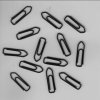
\includegraphics[width=0.4\textwidth]{figures/原始图像.png}
\caption{原始图像（100×100像素）}
\label{fig:original}
\end{figure}

图\ref{fig:fpga_display}展示了图像在FPGA开发板LCD屏幕上的实际显示效果，可以看到图像被4倍放大后居中显示在白色背景上。

\begin{figure}[H]
\centering
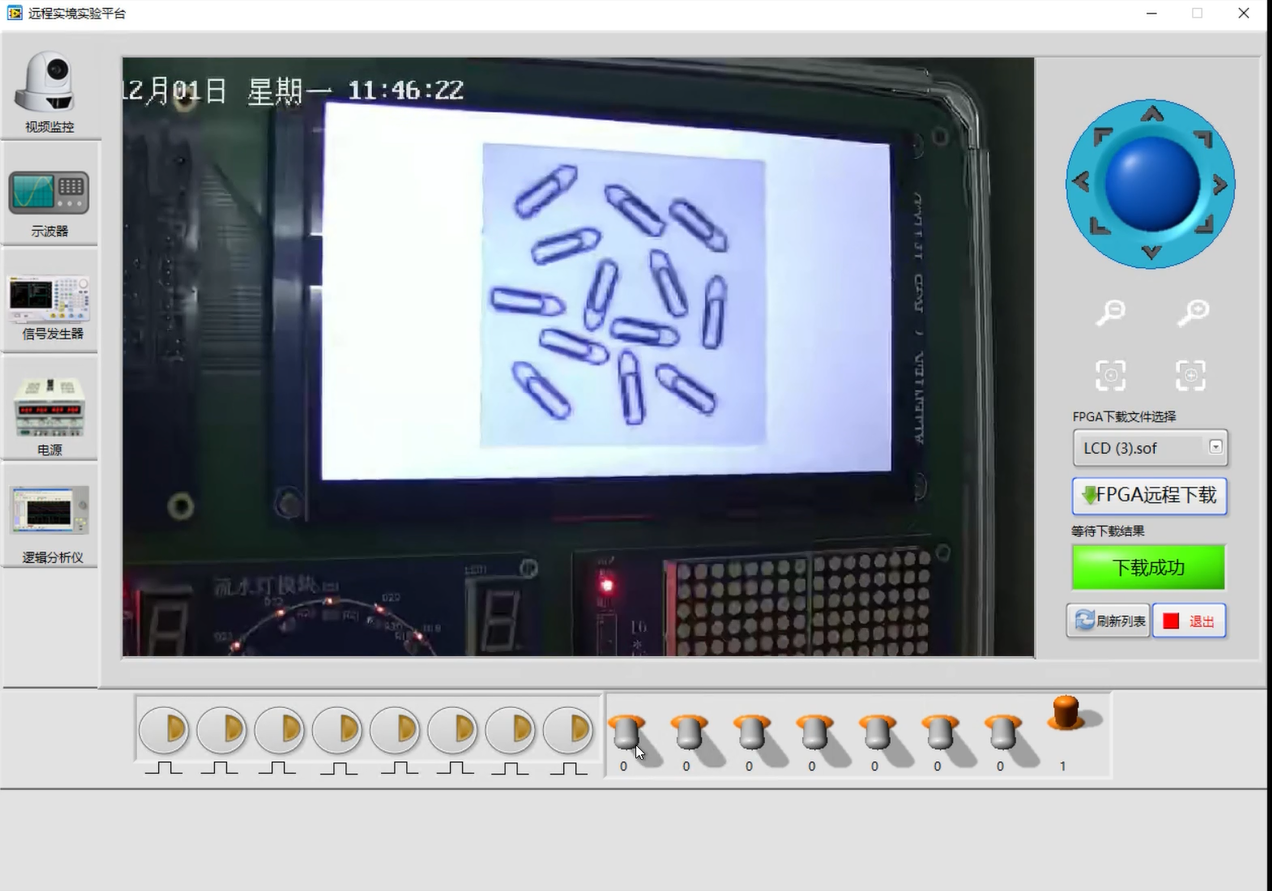
\includegraphics[width=0.6\textwidth]{figures/图像FPGA显示.png}
\caption{图像在FPGA LCD屏幕上的显示效果}
\label{fig:fpga_display}
\end{figure}

\subsection{Sobel边缘检测功能}

拨动Switch[0]后，系统使用Sobel算子进行边缘检测，检测结果以白底黑边的形式显示。Sobel算子对噪声有一定的抑制能力，检测出的边缘较为平滑。图\ref{fig:sobel}展示了Sobel边缘检测的效果。

\begin{figure}[H]
\centering
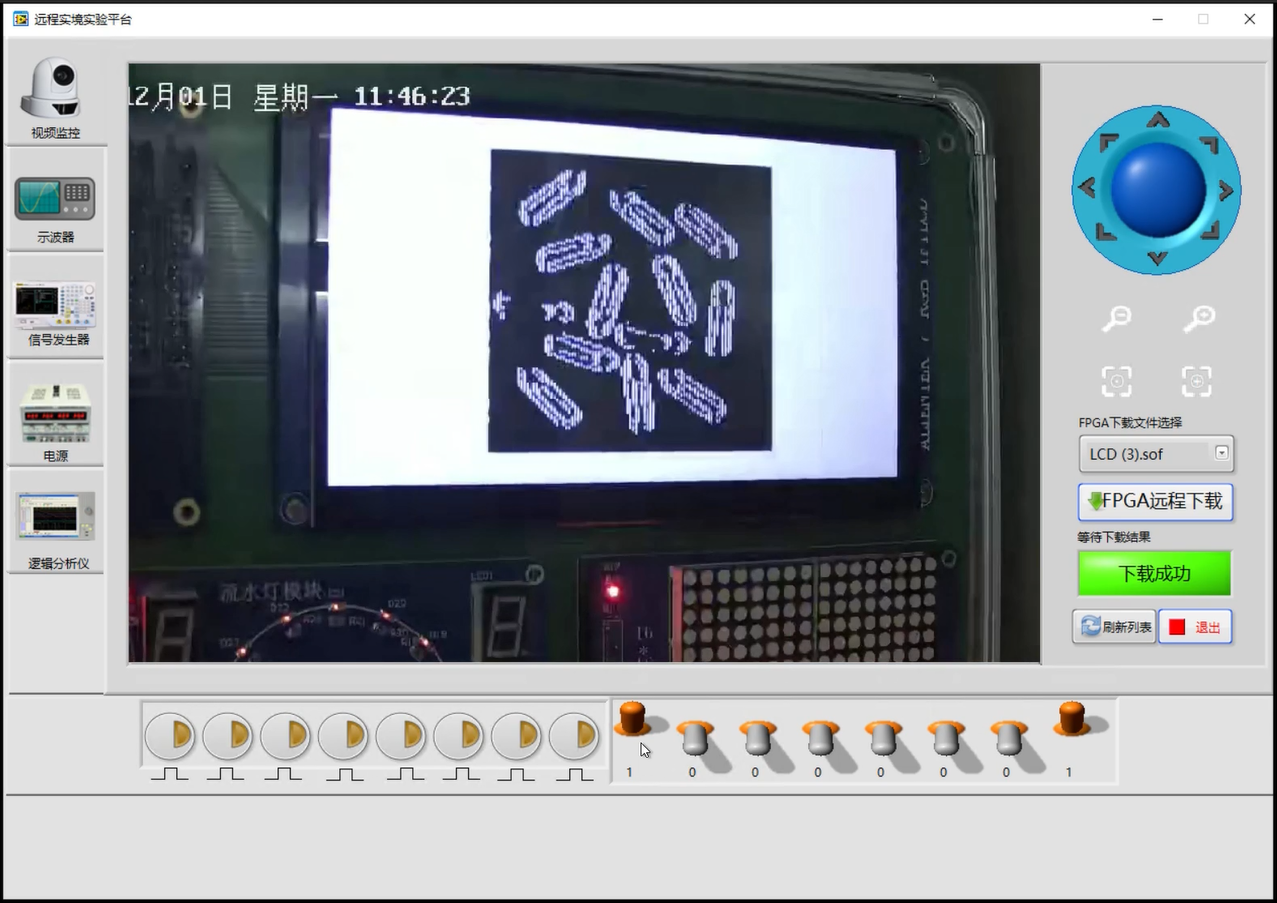
\includegraphics[width=0.5\textwidth]{figures/Sobel.png}
\caption{Sobel边缘检测效果}
\label{fig:sobel}
\end{figure}

\subsection{Prewitt边缘检测功能}

拨动Switch[1]后，系统使用Prewitt算子进行边缘检测。与Sobel相比，Prewitt检测出的边缘更为锐利，但对噪声更敏感。图\ref{fig:prewitt}展示了Prewitt边缘检测的效果。

\begin{figure}[H]
\centering
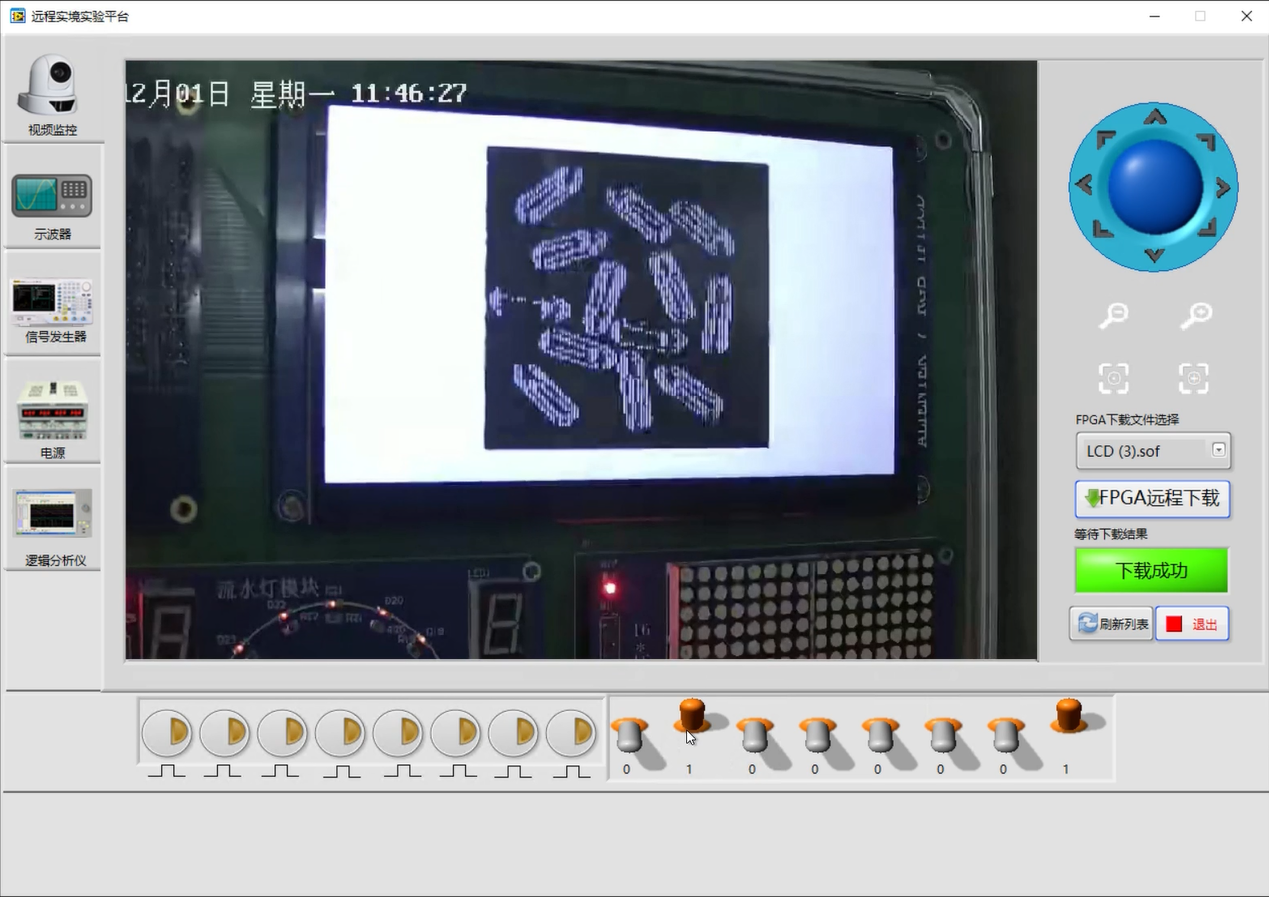
\includegraphics[width=0.5\textwidth]{figures/Prewitt.png}
\caption{Prewitt边缘检测效果}
\label{fig:prewitt}
\end{figure}

\subsection{功能切换测试}

通过实时切换拨码开关，可以即时观察不同边缘检测算法的效果差异，系统响应迅速，无明显延迟。对比图\ref{fig:sobel}和图\ref{fig:prewitt}可以发现，Sobel算子检测的边缘更加平滑连续，而Prewitt算子检测的边缘更加锐利清晰。

\section{结论}

本实验成功实现了基于FPGA的图像边缘检测系统，主要完成以下工作：

（1）实现了完整的图像处理流水线，包括坐标映射、图像缩放、RGB转灰度、3×3窗口构建等模块

（2）采用Sobel和Prewitt两种经典边缘检测算子，实现了与OpenCV软件库等效的硬件加速处理

（3）通过拨码开关实现算法的实时切换，便于对比不同算法的效果

（4）针对梯度幅值计算中绝对值和近似法的45°方向高估问题，提出了加权近似法的优化方案

本设计将软件图像处理算法硬件化，充分发挥了FPGA并行处理的优势，实现了实时图像边缘检测，对理解数字图像处理原理和FPGA设计方法具有重要的实践意义。

\section{参考文献}

\begin{enumerate}[label={[\arabic*]}]
    \item 冈萨雷斯. 数字图像处理（第三版）[M]. 电子工业出版社, 2011.
    \item OpenCV官方文档. Image Filtering — Sobel Derivatives[EB/OL]. https://docs.opencv.org/
    \item 夏宇闻. Verilog数字系统设计教程（第四版）[M]. 北京航空航天大学出版社, 2017.
    \item Intel Corporation. Cyclone IV Device Handbook[EB/OL]. https://www.intel.com/
\end{enumerate}

\newpage
\section*{附录：lcd\_display.v屏幕应用层程序}
\addcontentsline{toc}{section}{附录：源程序}

\begin{lstlisting}[caption={lcd\_display.v完整代码}]
module lcd_display(
  input        lcd_clk,        // LCD驱动时钟
  input        sys_rst_n,      // 复位信号
  input [3:0]  switches,       // B3,B2,B1,B0 开关输入
  input [10:0] pixel_xpos,     // 像素点横坐标(0-799)
  input [10:0] pixel_ypos,     // 像素点纵坐标(0-479)
  output reg [23:0] pixel_data // 像素点数据(RGB888)
);

//--
// Parameter definition
//---
localparam H_DISP = 11'd800;  // 水平分辨率
localparam V_DISP = 11'd480;  // 垂直分辨率

// Logo图片参数 (从LOGO.mif读取)
localparam IMG_WIDTH  = 11'd100;  // 原始图片宽度
localparam IMG_HEIGHT = 11'd100;  // 原始图片高度

// 缩放参数 (4倍放大: 100x100 -> 400x400)
localparam SCALE_FACTOR = 3'd4;   // 缩放倍数
localparam SCALED_WIDTH  = 11'd400;  // 缩放后宽度
localparam SCALED_HEIGHT = 11'd400;  // 缩放后高度

// 居中显示位置参数 (屏幕800x480，图像400x400)
localparam IMG_X = 11'd200;  // 图像左上角X坐标 (居中)
localparam IMG_Y = 11'd40;   // 图像左上角Y坐标 (居中)

// 颜色定义
localparam COLOR_BG = 24'hFFFFFF;  // 白色背景

// ROM相关信号
wire [13:0] rom_addr;
wire [23:0] rom_data;

wire [10:0] x_pos = (pixel_xpos == 11'd0) ? 11'd0 : pixel_xpos - 11'd1;
wire [10:0] y_pos = (pixel_ypos == 11'd0) ? 11'd0 : pixel_ypos - 11'd1;

wire in_active_area = (pixel_xpos >= 11'd1) && (pixel_xpos <= H_DISP) &&
                      (pixel_ypos >= 11'd1) && (pixel_ypos <= V_DISP);

// 判断当前像素是否在缩放后的图片范围内 (400x400)
wire [10:0] rel_x_scaled = x_pos - IMG_X;
wire [10:0] rel_y_scaled = y_pos - IMG_Y;
wire in_image = (x_pos >= IMG_X) && (x_pos < IMG_X + SCALED_WIDTH) && 
                (y_pos >= IMG_Y) && (y_pos < IMG_Y + SCALED_HEIGHT);

// 缩放算法: 最近邻插值
wire [6:0] src_x = rel_x_scaled[8:2];  // 除以4
wire [6:0] src_y = rel_y_scaled[8:2];  // 除以4

assign rom_addr = (src_y * 7'd100) + src_x;

//----
// Logo ROM实例化
//----------
logo_rom u_logo_rom (
  .address (rom_addr),
  .clock   (lcd_clk),
  .q       (rom_data)
);

// 寄存in_image信号以匹配ROM延迟
reg in_image_d1;
always @(posedge lcd_clk) begin
  in_image_d1 <= in_image;
end

//----------
// 图像处理流水线 - 边缘检测算法
//----------
wire [7:0] r = rom_data[23:16];
wire [7:0] g = rom_data[15:8];
wire [7:0] b = rom_data[7:0];

// 灰度化
wire [15:0] gray_calc = r * 77 + g * 150 + b * 29;
wire [7:0] gray = gray_calc[15:8];

//----------
// 3x3 像素窗口缓存
//----------
reg [7:0] line_buf0 [0:IMG_WIDTH-1];
reg [7:0] line_buf1 [0:IMG_WIDTH-1];

reg [7:0] p00, p01, p02;
reg [7:0] p10, p11, p12;
reg [7:0] p20, p21, p22;

reg in_image_d2, in_image_d3;
reg [6:0] src_x_d1, src_x_d2, src_x_d3;
reg [6:0] src_y_d1, src_y_d2, src_y_d3;

always @(posedge lcd_clk) begin
    in_image_d2 <= in_image_d1;
    in_image_d3 <= in_image_d2;
    src_x_d1 <= src_x;
    src_x_d2 <= src_x_d1;
    src_x_d3 <= src_x_d2;
    src_y_d1 <= src_y;
    src_y_d2 <= src_y_d1;
    src_y_d3 <= src_y_d2;
end

// 窗口构建
always @(posedge lcd_clk) begin
    if (in_image_d1) begin
        p02 <= p01; p01 <= p00; p00 <= line_buf0[src_x_d1];
        p12 <= p11; p11 <= p10; p10 <= line_buf1[src_x_d1];
        p22 <= p21; p21 <= p20; p20 <= gray;
        line_buf0[src_x_d1] <= line_buf1[src_x_d1];
        line_buf1[src_x_d1] <= gray;
    end
end

wire window_valid = in_image_d3 && (src_x_d3 >= 7'd2) && (src_y_d3 >= 7'd2);

//----------
// Sobel 边缘检测
//----------
wire signed [10:0] sobel_gx_row0 = $signed({3'b0, p02}) - $signed({3'b0, p00});
wire signed [10:0] sobel_gx_row1 = ($signed({3'b0, p12}) - $signed({3'b0, p10})) <<< 1;
wire signed [10:0] sobel_gx_row2 = $signed({3'b0, p22}) - $signed({3'b0, p20});
wire signed [11:0] sobel_gx = sobel_gx_row0 + sobel_gx_row1 + sobel_gx_row2;

wire signed [10:0] sobel_gy_top = $signed({3'b0, p00}) + ($signed({3'b0, p01}) <<< 1) + $signed({3'b0, p02});
wire signed [10:0] sobel_gy_bot = $signed({3'b0, p20}) + ($signed({3'b0, p21}) <<< 1) + $signed({3'b0, p22});
wire signed [11:0] sobel_gy = sobel_gy_top - sobel_gy_bot;

wire [11:0] sobel_gx_abs = (sobel_gx < 0) ? -sobel_gx : sobel_gx;
wire [11:0] sobel_gy_abs = (sobel_gy < 0) ? -sobel_gy : sobel_gy;
wire [12:0] sobel_mag_full = sobel_gx_abs + sobel_gy_abs;
wire [7:0] sobel_mag = (sobel_mag_full > 13'd2040) ? 8'd255 : sobel_mag_full[10:3];
wire [23:0] data_sobel = (window_valid && sobel_mag > 8'd30) ? 24'h000000 : 24'hFFFFFF;

//----------
// Prewitt 边缘检测
//----------
wire signed [10:0] prewitt_gx_row0 = $signed({3'b0, p02}) - $signed({3'b0, p00});
wire signed [10:0] prewitt_gx_row1 = $signed({3'b0, p12}) - $signed({3'b0, p10});
wire signed [10:0] prewitt_gx_row2 = $signed({3'b0, p22}) - $signed({3'b0, p20});
wire signed [11:0] prewitt_gx = prewitt_gx_row0 + prewitt_gx_row1 + prewitt_gx_row2;

wire signed [10:0] prewitt_gy_top = $signed({3'b0, p00}) + $signed({3'b0, p01}) + $signed({3'b0, p02});
wire signed [10:0] prewitt_gy_bot = $signed({3'b0, p20}) + $signed({3'b0, p21}) + $signed({3'b0, p22});
wire signed [11:0] prewitt_gy = prewitt_gy_top - prewitt_gy_bot;

wire [11:0] prewitt_gx_abs = (prewitt_gx < 0) ? -prewitt_gx : prewitt_gx;
wire [11:0] prewitt_gy_abs = (prewitt_gy < 0) ? -prewitt_gy : prewitt_gy;
wire [12:0] prewitt_mag_full = prewitt_gx_abs + prewitt_gy_abs;
wire [7:0] prewitt_mag = (prewitt_mag_full > 13'd1530) ? 8'd255 : prewitt_mag_full[10:3];
wire [23:0] data_prewitt = (window_valid && prewitt_mag > 8'd25) ? 24'h000000 : 24'hFFFFFF;

//----------
// 像素显示逻辑
//----------
always @(posedge lcd_clk or negedge sys_rst_n) begin
  if (!sys_rst_n) begin
    pixel_data <= COLOR_BG;
  end else begin
    if (!in_active_area) begin
      pixel_data <= COLOR_BG;
    end else begin
      if (in_image_d1) begin
        case (switches[1:0])
            2'b01: pixel_data <= data_sobel;    // Switch[0]: Sobel
            2'b10: pixel_data <= data_prewitt;  // Switch[1]: Prewitt
            default: pixel_data <= rom_data;    // Default: 原图
        endcase
      end else begin
        pixel_data <= COLOR_BG;
      end
    end
  end
end

endmodule
\end{lstlisting}

\end{document}
